\documentclass[12pt, titlepage]{article}

\usepackage{fullpage}
\usepackage[round]{natbib}
\usepackage{multirow}
\usepackage{booktabs}
\usepackage{tabularx}
\usepackage{graphicx}
\usepackage{float}
\usepackage{hyperref}
\usepackage{soul}

\hypersetup{
    colorlinks,
    citecolor=black,
    filecolor=black,
    linkcolor=red,
    urlcolor=blue
}
\usepackage[round]{natbib}

\newcounter{acnum}
\newcommand{\actheacnum}{AC\theacnum}
\newcommand{\acref}[1]{AC\ref{#1}}

\newcounter{ucnum}
\newcommand{\uctheucnum}{UC\theucnum}
\newcommand{\uref}[1]{UC\ref{#1}}

\newcounter{mnum}
\newcommand{\mthemnum}{M\themnum}
\newcommand{\mref}[1]{M\ref{#1}}

\title{SE 3XA3: Software Requirements Specification\\PocketSaver}

\author{Team 12, 
		\\ Mevin Mathew , mathem1 , 400012057
		\\ Shalmi Patel , patels19 , 400023762
		\\ Diya Mathews , mathewsd , 400014156
}

\date{\today}

%% Comments

\usepackage{color}

\newif\ifcomments\commentstrue

\ifcomments
\newcommand{\authornote}[3]{\textcolor{#1}{[#3 ---#2]}}
\newcommand{\todo}[1]{\textcolor{red}{[TODO: #1]}}
\else
\newcommand{\authornote}[3]{}
\newcommand{\todo}[1]{}
\fi

\newcommand{\wss}[1]{\authornote{blue}{SS}{#1}}
\newcommand{\ds}[1]{\authornote{red}{DS}{#1}}
\newcommand{\mj}[1]{\authornote{red}{MSN}{#1}}
\newcommand{\mh}[1]{\authornote{red}{MH}{#1}}
\newcommand{\cm}[1]{\authornote{red}{CM}{#1}}


% team members should be added for each team, like the following
% all comments left by the TAs or the instructor should be addressed
% by a corresponding comment from the Team

\newcommand{\tm}[1]{\authornote{magenta}{Team}{#1}}


\begin{document}

\maketitle

\pagenumbering{roman}
\tableofcontents
\listoftables
\listoffigures

\begin{table}[bp]
\caption{\bf Revision History}
\begin{tabularx}{\textwidth}{p{3cm}p{2cm}X}
\toprule {\bf Date} & {\bf Version} & {\bf Notes}\\
\midrule
November 9 & 1.0 & Made an outline of all the modules in PocketSaver and started brainstorming the design\\
November 10 & 1.1 & Finished the design document\\
\midrule
December 6 & 1.2 & Rev1 Submission\\
\bottomrule
\end{tabularx}
\end{table}

\newpage

\pagenumbering{arabic}

\section{Introduction}

Decomposing a system into modules is a commonly accepted approach to developing
software.  A module is a work assignment for a programmer or programming
team (Parnas et al., 1984).  We advocate a decomposition
based on the principle of information hiding (Parnas, 1972).  This
principle supports design for change, because the ``secrets'' that each module
hides represent likely future changes.  Design for change is valuable in SC,
where modifications are frequent, especially during initial development as the
solution space is explored.  

Our design follows the rules layed out by Parnas et al. (1984), as follows:
\begin{itemize}
\item System details that are likely to change independently should be the
  secrets of separate modules.
\item Each data structure is used in only one module.
\item Any other program that requires information stored in a module's data
  structures must obtain it by calling access programs belonging to that module.
\end{itemize}

After completing the first stage of the design, the Software Requirements
Specification (SRS), the Module Guide (MG) is developed~\citep{ParnasEtAl1984}. The MG
specifies the modular structure of the system and is intended to allow both
designers and maintainers to easily identify the parts of the software.  The
potential readers of this document are as follows:

\begin{itemize}
\item New project members: This document can be a guide for a new project member
  to easily understand the overall structure and quickly find the
  relevant modules they are searching for.
\item Maintainers: The hierarchical structure of the module guide improves the
  maintainers' understanding when they need to make changes to the system. It is
  important for a maintainer to update the relevant sections of the document
  after changes have been made.
\item Designers: Once the module guide has been written, it can be used to
  check for consistency, feasibility and flexibility. Designers can verify the
  system in various ways, such as consistency among modules, feasibility of the
  decomposition, and flexibility of the design.
\end{itemize}

The rest of the document is organized as follows. Section
\ref{SecChange} lists the anticipated and unlikely changes of the software
requirements. Section \ref{SecMH} summarizes the module decomposition that
was constructed according to the likely changes. Section \ref{SecConnection}
specifies the connections between the software requirements and the
modules. Section \ref{SecMD} gives a detailed description of the
modules. Section \ref{SecTM} includes two traceability matrices. One checks
the completeness of the design against the requirements provided in the SRS. The
other shows the relation between anticipated changes and the modules. Section
\ref{SecUse} describes the use relation between modules.

\section{Anticipated and Unlikely Changes} \label{SecChange}

This section lists possible changes to the system. According to the likeliness
of the change, the possible changes are classified into two
categories. Anticipated changes are listed in Section \ref{SecAchange}, and
unlikely changes are listed in Section \ref{SecUchange}.

\subsection{Anticipated Changes} \label{SecAchange}

Anticipated changes are the source of the information that is to be hidden
inside the modules. Ideally, changing one of the anticipated changes will only
require changing the one module that hides the associated decision. The approach
adapted here is called design for
change.

\begin{description}
\item[\refstepcounter{acnum} \actheacnum \label{ac1}:] The hardware on which the software is running.
\item[\refstepcounter{acnum} \actheacnum \label{ac2}:] Application user interface layout on various devices (Responsivity).
\item[\refstepcounter{acnum} \actheacnum \label{ac3}:] User interface appearance and colour scheme.
\end{description}

\subsection{Unlikely Changes} \label{SecUchange}

The module design should be as general as possible. However, a general system is
more complex. Sometimes this complexity is not necessary. Fixing some design
decisions at the system architecture stage can simplify the software design. If
these decision should later need to be changed, then many parts of the design
will potentially need to be modified. Hence, it is not intended that these
decisions will be changed.

\begin{description}
\item[\refstepcounter{ucnum} \uctheucnum \label{uc1}:] Input device (On screen keyboard).
\item[\refstepcounter{ucnum} \uctheucnum \label{uc2}:] Output device (device screen).
\item[\refstepcounter{ucnum} \uctheucnum \label{uc3}:] Transaction entries updating and new entries logic.
\item[\refstepcounter{ucnum} \uctheucnum \label{uc4}:] Total expense calculation logic.
\end{description}

\section{Module Hierarchy} \label{SecMH}

This section provides an overview of the module design. Modules are summarized
in a hierarchy decomposed by secrets in Table \ref{TblMH}. The modules listed
below, which are leaves in the hierarchy tree, are the modules that will
actually be implemented.

\begin{description}
\item [\refstepcounter{mnum} \mthemnum \label{m1}:] CustomImageCell Module
\item [\refstepcounter{mnum} \mthemnum \label{m2}:] Transaction Model Module
\item [\refstepcounter{mnum} \mthemnum \label{m3}:] ApiSV \textcolor{blue}{\st{Module}} model
\item [\refstepcounter{mnum} \mthemnum \label{m4}:] HomePage ViewModel Module
\item [\refstepcounter{mnum} \mthemnum \label{m5}:] TransactionPage ViewModel Module
\item [\refstepcounter{mnum} \mthemnum \label{m6}:] \textcolor{blue}{\st{ SettingsPage ViewModel Module}}
\item [\refstepcounter{mnum} \mthemnum \label{m7}:] \textcolor{blue}{\st{ PageActivityIndicator Module}}
\item [\refstepcounter{mnum} \mthemnum \label{m8}:] TintedImage Module
\item [\refstepcounter{mnum} \mthemnum \label{m9}:] TransactionListCell Module
\item [\refstepcounter{mnum} \mthemnum \label{m10}:] TransactionListPage
\item [\refstepcounter{mnum} \mthemnum \label{m11}:] AboutPage Module
\item [\refstepcounter{mnum} \mthemnum \label{m12}:] HomePage Module
\item [\refstepcounter{mnum} \mthemnum \label{m13}:] GroupedMasterPageItem Module
\item [\refstepcounter{mnum} \mthemnum \label{m14}:] MasterPageItem Module
\item [\refstepcounter{mnum} \mthemnum \label{m15}:] MainMasterDetailPage Module
\item [\refstepcounter{mnum} \mthemnum \label{m16}:] MainMenuPage Module
\item [\refstepcounter{mnum} \mthemnum \label{m17}:]\textcolor{blue}{StorageSV model}

\end{description}


\begin{table}[h!]
\centering
\begin{tabular}{p{0.3\textwidth} p{0.6\textwidth}}
\toprule
\textbf{Level 1} & \textbf{Level 2}\\
\midrule

{Hardware-Hiding Module} & CustomImageCell Module \\
& TintedImage Module\\
& GroupedMasterPageItem Module\\
& MasterPageItem Module\\
& MainMasterDetailPage Module\\
& MainMenuPage Module\\
\midrule

\multirow{7}{0.3\textwidth}{Behaviour-Hiding Module} & Transaction Model Module\\
& ApiSV Module\\
& Home ViewModel Module\\
& Transaction ViewModel Module\\
& Settings ViewModel Module\\
& PageActivityIndicator Module\\
& TransactionList Cell Module\\ 
& TransactionListPage Module\\
& AboutPage Module\\
& HomePage Module\\
\midrule

\multirow{1}{0.3\textwidth}{Software Decision Module} & {}\\
\bottomrule

\end{tabular}
\caption{Module Hierarchy}
\label{TblMH}
\end{table}

\section{Connection Between Requirements and Design} \label{SecConnection}

The design of the system is intended to satisfy the requirements developed in
the SRS. In this stage, the system is decomposed into modules. The connection
between requirements and modules is listed in Table \ref{TblRT}.

\section{Module Decomposition} \label{SecMD}

Modules are decomposed according to the principle of ``information hiding''
proposed by \citet{ParnasEtAl1984}. The \emph{Secrets} field in a module
decomposition is a brief statement of the design decision hidden by the
module. The \emph{Services} field specifies \emph{what} the module will do
without documenting \emph{how} to do it. For each module, a suggestion for the
implementing software is given under the \emph{Implemented By} title. If the
entry is \emph{OS}, this means that the module is provided by the operating
system or by standard programming language libraries.  Also indicate if the
module will be implemented specifically for the software.

Only the leaf modules in the
hierarchy have to be implemented. If a dash (\emph{--}) is shown, this means
that the module is not a leaf and will not have to be implemented. Whether or
not this module is implemented depends on the programming language
selected.

\subsection{Hardware Hiding Modules}
\subsubsection{CustomImageCell Module(\mref{m1})}
\begin{description}
\item[Secrets:] \textcolor{blue}{\st{Get}}Colours from module
\item[Services:]Allows custom cells to have tinted images
\item[Implemented By:] CustomImageCell.cs
\end{description}

\subsubsection{TintedImage Module(\mref{m7})}
\begin{description}
\item[Secrets:]\textcolor{blue}{\st{Get}} Colours from module
\item[Services:]A custom image that allows for image colour tinting for the main menu images and various other pages
\item[Implemented By:] TintedImage.cs
\end{description}

\subsubsection{GroupedMasterPageItem Module(\mref{m13})}
\begin{description}
\item[Secrets:] \textcolor{blue}{\st{How the MasterPageItem is grouped together}} MasterPageItem grouped layout
\item[Services:]Groups the items in the master page into Modules for the MainMenuPage list
\item[Implemented By:] GroupedMasterPageItem.cs
\end{description}

\subsubsection{MasterPageItem Module(\mref{m14})}
\begin{description}
\item[Secrets:] How each page is created for each view
\item[Services:]Determines the instances of pages to be loaded upon user selection
\item[Implemented By:] MasterPageItem.cs
\end{description}

\subsubsection{MainMasterDetailPage Module(\mref{m15})}
\begin{description}
\item[Secrets:]\textcolor{blue}{\st{How the}} Navigation flows from page to page using MasterDetail layout
\item[Services:]Displays the master detail format for the pages of the application
Module that creates an instance of a master detail format for the pages
\item[Implemented By:]  MainMasterDetailPage.xaml, MainMasterDetailPage.cs
\end{description}

\subsubsection{MainMenuPage Module(\mref{m16})}
\begin{description}
\item[Secrets:] \textcolor{blue}{\st{How the MainMenu is laid out}} \textcolor{blue}{ Layout of the MainMenu}
\item[Services:]Module that displays the list of all pages within the application
\item[Implemented By:] MainMenuPage.xaml, MainMenuPage.cs
\end{description}

\subsection{Behaviour-Hiding Module}
\subsubsection{ApiSV Model(\mref{m3})}
\begin{description}
\item[Secrets:] \textcolor{blue}{\st{How the GET and POST requests are made}}\textcolor{blue}{GET and POST requests}
\item[Services:] API Service that allows the application to use GET and POST requests to retrieve and add data to the online database
\item[Implemented By:] ApiSV.cs
\end{description}

\subsubsection{Home ViewModel Module(\mref{m4})}
\begin{description}
\item[Secrets:] Data Retrieval from the ApiSV module
\item[Services:] Does all back end data retrieval for the Home page to be used within the HomePage view
\item[Implemented By:] HomeViewModel.cs
\end{description}

\subsubsection{Transaction ViewModel Module(\mref{m5})}
\begin{description}
\item[Secrets:] Data Retrieval from the ApiSV module
\item[Services:] Does all of the back end data retrieval for the TransactionPage view
\item[Implemented By:] TransactionViewModel.cs
\end{description}

\subsubsection{StroageSV Model(\mref{m6})}
\begin{description}
\item[Secrets:] Data Retrieval from the ApiSV
\item[Services:] Saves any local settings created by the user to be used for the SettingsPage view
\item[Implemented By:] SettingsViewModel.cs
\end{description}

\subsubsection{TransactionList Cell Module (\mref{m9})}
\begin{description}
\item[Secrets:] How the ListCell is formatted for the ListView in the TransactionListPage
\item[Services:] Displays the data for each transaction as a specific format determined by the developer
\item[Implemented By:] TransactionListCell.cs
\end{description}

\subsubsection{TransactionListPage Module (\mref{m10})} 
\begin{description} 
\item[Secrets:] The data \textcolor{blue}{\st{is displayed}} \textcolor{blue}{received} from the Transaction ViewModel 
\item[Services:] Displaying the data from the TransactionViewModel onto the UI View for the user
\item[Implemented By:] TransactionListPage.xaml, TransactionListPage.cs 
\end{description}

\subsubsection{AboutPage Module(\mref{m11})}
\begin{description} 
\item[Secrets:] N/A 
\item[Services:] Dispays the title, version and brief description of the PocketSaver Application 
\item[Implemented By:] AboutPage.xaml, AboutPage.cs 
\end{description}

\subsubsection{HomePage Module (\mref{m12})} 
\begin{description}
\item[Secrets:] Data \textcolor{blue}{\st{is displayed}} \textcolor{blue}{received} from the HomePageViewModel to the UI view
\item[Services:] Displays the data from the HomePageViewModel to the UI View for the user
\item[Implemented By:] HomePage.xaml, HomePage.cs 
\end{description}

\section{Traceability Matrix} \label{SecTM}

This section shows two traceability matrices: between the modules and the
requirements and between the modules and the anticipated changes.

% the table should use mref, the requirements should be named, use something
% like fref
\begin{table}[H]
\centering
\begin{tabular}{p{0.2\textwidth} p{0.6\textwidth}}
\toprule
\textbf{Req.} & \textbf{Modules}\\
\midrule
FR1 & \mref{m9}, \mref{m7}\\
FR2 & \mref{m9}, \mref{m7}, \mref{m11}, \mref{m12}\\
FR3 & \mref{m7}, \mref{m11}, \mref{m12}\\
FR4 & \mref{m7}\\
\bottomrule
\end{tabular}
\caption{Trace Between Requirements and Modules}
\label{TblRT}
\end{table}

\begin{table}[H]
\centering
\begin{tabular}{p{0.2\textwidth} p{0.6\textwidth}}
\toprule
\textbf{AC} & \textbf{Modules}\\
\midrule
\acref{ac1} & \mref{m1}, \mref{m2}, \mref{m4}, \mref{m5}, \mref{m6}, \mref{m10}, \mref{m16}\\
\acref{ac2} & \mref{m4}, \mref{m5}, \mref{m10}, \mref{m11}, \mref{m16}\\
\acref{ac3} & \mref{m4}, \mref{m5}, \mref{m10}, \mref{m11}, \mref{m16}\\
\bottomrule
\end{tabular}
\caption{Trace Between Anticipated Changes and Modules}
\label{TblACT}
\end{table}

\section{Use Hierarchy Between Modules} \label{SecUse}

In this section, the uses hierarchy between modules is
provided. Parnas1978 said of two programs A and B that A {\em uses} B if
correct execution of B may be necessary for A to complete the task described in
its specification. That is, A {\em uses} B if there exist situations in which
the correct functioning of A depends upon the availability of a correct
implementation of B.  Figure \ref{FigUH} illustrates the use relation between
the modules. It can be seen that the graph is a directed acyclic graph
(DAG). Each level of the hierarchy offers a testable and usable subset of the
system, and modules in the higher level of the hierarchy are essentially simpler
because they use modules from the lower levels.

\begin{figure}[H]
\centering
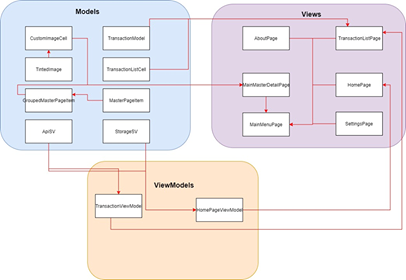
\includegraphics[width=0.7\textwidth]{UsesHierarchy.png}
\caption{Use hierarchy among modules}
\label{FigUH}
\end{figure}


\bibliographystyle {plainnat}
\bibliography {MG}

\end{document}
